\documentclass[11pt]{article}
\usepackage[T1]{fontenc}
\usepackage{geometry, changepage}
\usepackage{amsmath, amssymb, amsthm, bm}
\usepackage{physics}
\usepackage{hyperref}

\usepackage{tikz}
\usetikzlibrary{arrows.meta}
\hypersetup{colorlinks=true, linkcolor=blue, urlcolor=cyan}
\setlength{\parindent}{0pt}
\setlength{\parskip}{5pt}

\newtheorem{theorem}{Theorem}
\newtheorem{lemma}{Lemma}
\newtheorem{claim}{Claim}
\newtheorem*{theorem*}{Theorem}
\newtheorem*{lemma*}{Lemma}
\newtheorem*{claim*}{Claim}

\renewcommand{\vec}[1]{\mathbf{#1}}
\newcommand{\uvec}[1]{\mathop{} \!\hat{\mathbf{#1}}}
\newcommand{\mat}[1]{\mathbf{#1}}
\newcommand{\tensor}[1]{\mathsf{#1}}

\renewcommand{\div}{\nabla \cdot}
\renewcommand{\curl}{\nabla \cross}
\renewcommand{\grad}{\nabla}
\renewcommand{\laplacian}{\nabla^{2}}

\title{MATH-UA 140: Assignment 5}
\author{James Pagan, October 2023}
\date{Professor Raquépas}

% --------------------------------------------- %

\begin{document}

\maketitle
\tableofcontents

% --------------------------------------------- %

\section{Problem 1}

\textbf{Part (a)}: We have that
\[
	A^{2} = \begin{bmatrix} 0 & 1 & 1 & 1 \\ 0 & 0 & 1 & 0 \\ 1 & 0 & 1 & 1 \\ 0 & 1 & 1 & 0 \end{bmatrix} \begin{bmatrix} 0 & 1 & 1 & 1 \\ 0 & 0 & 1 & 0 \\ 1 & 0 & 1 & 1 \\ 0 & 1 & 1 & 0 \end{bmatrix} = \begin{bmatrix} 1 & 1 & 3 & 1 \\ 1 & 0 & 1 & 1 \\ 1 & 2 & 3 & 2 \\ 1 & 0 & 2 & 1 \end{bmatrix}.
\]
\textbf{Part (b)}: We have that
\[
	A^{3} = A^{2} A = \begin{bmatrix} 1 & 1 & 3 & 1 \\ 1 & 0 & 1 & 1 \\ 1 & 2 & 3 & 2 \\ 1 & 0 & 2 & 1 \end{bmatrix} \begin{bmatrix} 0 & 1 & 1 & 1 \\ 0 & 0 & 1 & 0 \\ 1 & 0 & 1 & 1 \\ 0 & 1 & 1 & 0 \end{bmatrix} = \begin{bmatrix} 3 & 2 & 6 & 4 \\ 1 & 2 & 3 & 2 \\ 3 & 3 & 8 & 4 \\ 2 & 2 & 4 & 3 \end{bmatrix}.
\]
The positivity of all entries implies that there exist paths of length $3$ between any two nodes of the graph.

\textbf{Part (c)}: Consider the graph pictured below (which I made using tikz, unfortunately):

\qquad \qquad \qquad 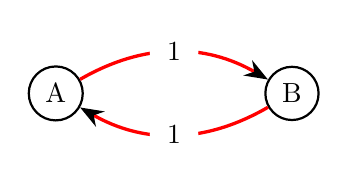
\begin{tikzpicture}
	\begin{scope}[every node/.style={circle,thick,draw}]
    	\node (A) at (0,0) {A};
    	\node (B) at (3,0) {B};
	\end{scope}
	\begin{scope}[>={Stealth[black]},
              every node/.style={fill=white,circle},
              every edge/.style={draw=red,very thick}]
    	\path [->] (A) edge[bend left=30] node {$1$} (B);
    	\path [->] (B) edge[bend left=30] node {$1$} (A);
\end{scope}
\end{tikzpicture}

Observe that there exists a path between any choice of nodes. However, a path connects $A$ to $B$ or $B$ to $A$ if and only if take an odd number of steps --- and comparatively, a path connects $A$ to $A$ or $B$ to $B$ if and only if it takes an even number of steps.

Thus a common length cannot exist --- if we suppose it does for contradiction, its parity implies it can only account for \textit{one} of the two types of paths discussed above.

\textbf{Part (d)}: Its corresponding adjacency matrix is
\[
	A = \begin{bmatrix} 0 & 1 \\ 1 & 0 \end{bmatrix},
\]
and its powers are
\begin{align*}
	A^{2} &= \begin{bmatrix} 0 & 1 \\ 1 & 0 \end{bmatrix} \begin{bmatrix} 0 & 1 \\ 1 & 0 \end{bmatrix} = \begin{bmatrix} 0 & 1 \\ 1 & 0 \end{bmatrix} \\
	A^{3} &= A^{2} A = \begin{bmatrix} 0 & 1 \\ 1 & 0 \end{bmatrix} \begin{bmatrix} 0 & 1 \\ 1 & 0 \end{bmatrix} = \begin{bmatrix} 0 & 1 \\ 1 & 0 \end{bmatrix} \\
	A^{4} &= A^{3}A = \begin{bmatrix} 0 & 1 \\ 1 & 0 \end{bmatrix} \begin{bmatrix} 0 & 1 \\ 1 & 0 \end{bmatrix} = \begin{bmatrix} 0 & 1 \\ 1 & 0 \end{bmatrix}.
\end{align*}

\textbf{Part (e)}: The transpose of the adjacency matrix of a directed graph describes 

the $\boxed{\text{graph created by flipping the directions of all its arrows}}$.

% --------------------------------------------- %

\section{Problem 2}

\textbf{Part (a)}: The column rank of $M$ is clearly $2$, as the first and second coulums are independent, but the third and the second are not. Thus, the null space of $M$ is the span of a single vector. One such vector is $(0, 2, -1)$, as
\[
	\begin{bmatrix} -2 & 0 & 0 \\ 0 & 1 & -2 \\ 0 & 3 & -6 \end{bmatrix} \begin{bmatrix} 0 \\ 2 \\ 1 \end{bmatrix} = \begin{bmatrix} 0 \\ 2 - 2 \\ 6 - 6 \end{bmatrix} = \begin{bmatrix} 0 \\ 0 \\ 0 \end{bmatrix}.
\]
This vector is thus a basis of the null space of $M$.

\textbf{Part (b)}: The row rank of $M$ is clearly $2$, as the first and second rows are independent, but the third and second are not. As the first and second rows constitute a list of $2$ independent vectors in the row space of $M$, they must be a basis; these two vectors are
\[
	\begin{bmatrix} -2 \\ 0 \\ 0 \end{bmatrix} \qquad \text{and} \qquad \begin{bmatrix} 0 \\ 1 \\ -2 \end{bmatrix}.
\]
\textbf{Part (c)}: We have that for all $\mu_{1}, \mu_{2} \in \mathbb{R}$,
\begin{align*}
	\left( \lambda \begin{bmatrix} 0 \\ 2 \\ 1 \end{bmatrix} \right) \cdot \left( \mu_{1} \begin{bmatrix} -2 \\ 0 \\ 0  \end{bmatrix} + \mu_{2} \begin{bmatrix} 0 \\ 1 \\ -2 \end{bmatrix} \right) &= \lambda \mu_{1} \begin{bmatrix} 0 \\ 2 \\ 1 \end{bmatrix} \cdot \begin{bmatrix} -2 \\ 0 \\ 0 \end{bmatrix} + \lambda \mu_{2} \begin{bmatrix} 0 \\ 2 \\ 1 \end{bmatrix} \cdot \begin{bmatrix} 0 \\ 1 \\ -2 \end{bmatrix} \\ 
	&= \lambda \mu_{1} (0) + \lambda \mu_{2} (0) \\
	&= 0.
\end{align*}
Thus, $\boxed{\text{the row space of $M$ is the orthogonal complement of the null space of $M$}}$ with respect to $\mathbb{R}^{3}$.

% --------------------------------------------- %

\end{document}
